\section{Introduction}

\begin{definition}[\textit{Computer performance}]
    Computer performance refers to the overall effectiveness of a computer system, considering factors such as throughput, individual response time, and availability.
\end{definition}
Computer performance can be evaluated by measuring the amount of useful work a computer system or network accomplishes within a specific time frame and resource allocation.

Systems are often validated primarily against functional requirements, with less emphasis on quality requirements early in the development process. 
This is partly due to limited initial information about system quality. 
However, understanding quality is crucial for managing both cost and performance throughout the system's lifecycle. 
This understanding is essential not only during the design and sizing phases but also as the system evolves.

\subsection{System quality evaluation}
System quality evaluation involves both intuition and trend extrapolation, allowing for quick and flexible assessments based on gut feelings and projected patterns. 
However, experts with sufficient experience in these areas are scarce, and the accuracy of their predictions can sometimes be questionable.

Experimentation is a highly beneficial and often preferred method for evaluating alternatives. 
While experiments provide detailed insights into system behavior under specific conditions, they can be costly and labor-intensive, lacking broader generalizations.
Despite these limitations, experiments typically offer high accuracy.
\begin{figure}[H]
    \centering
    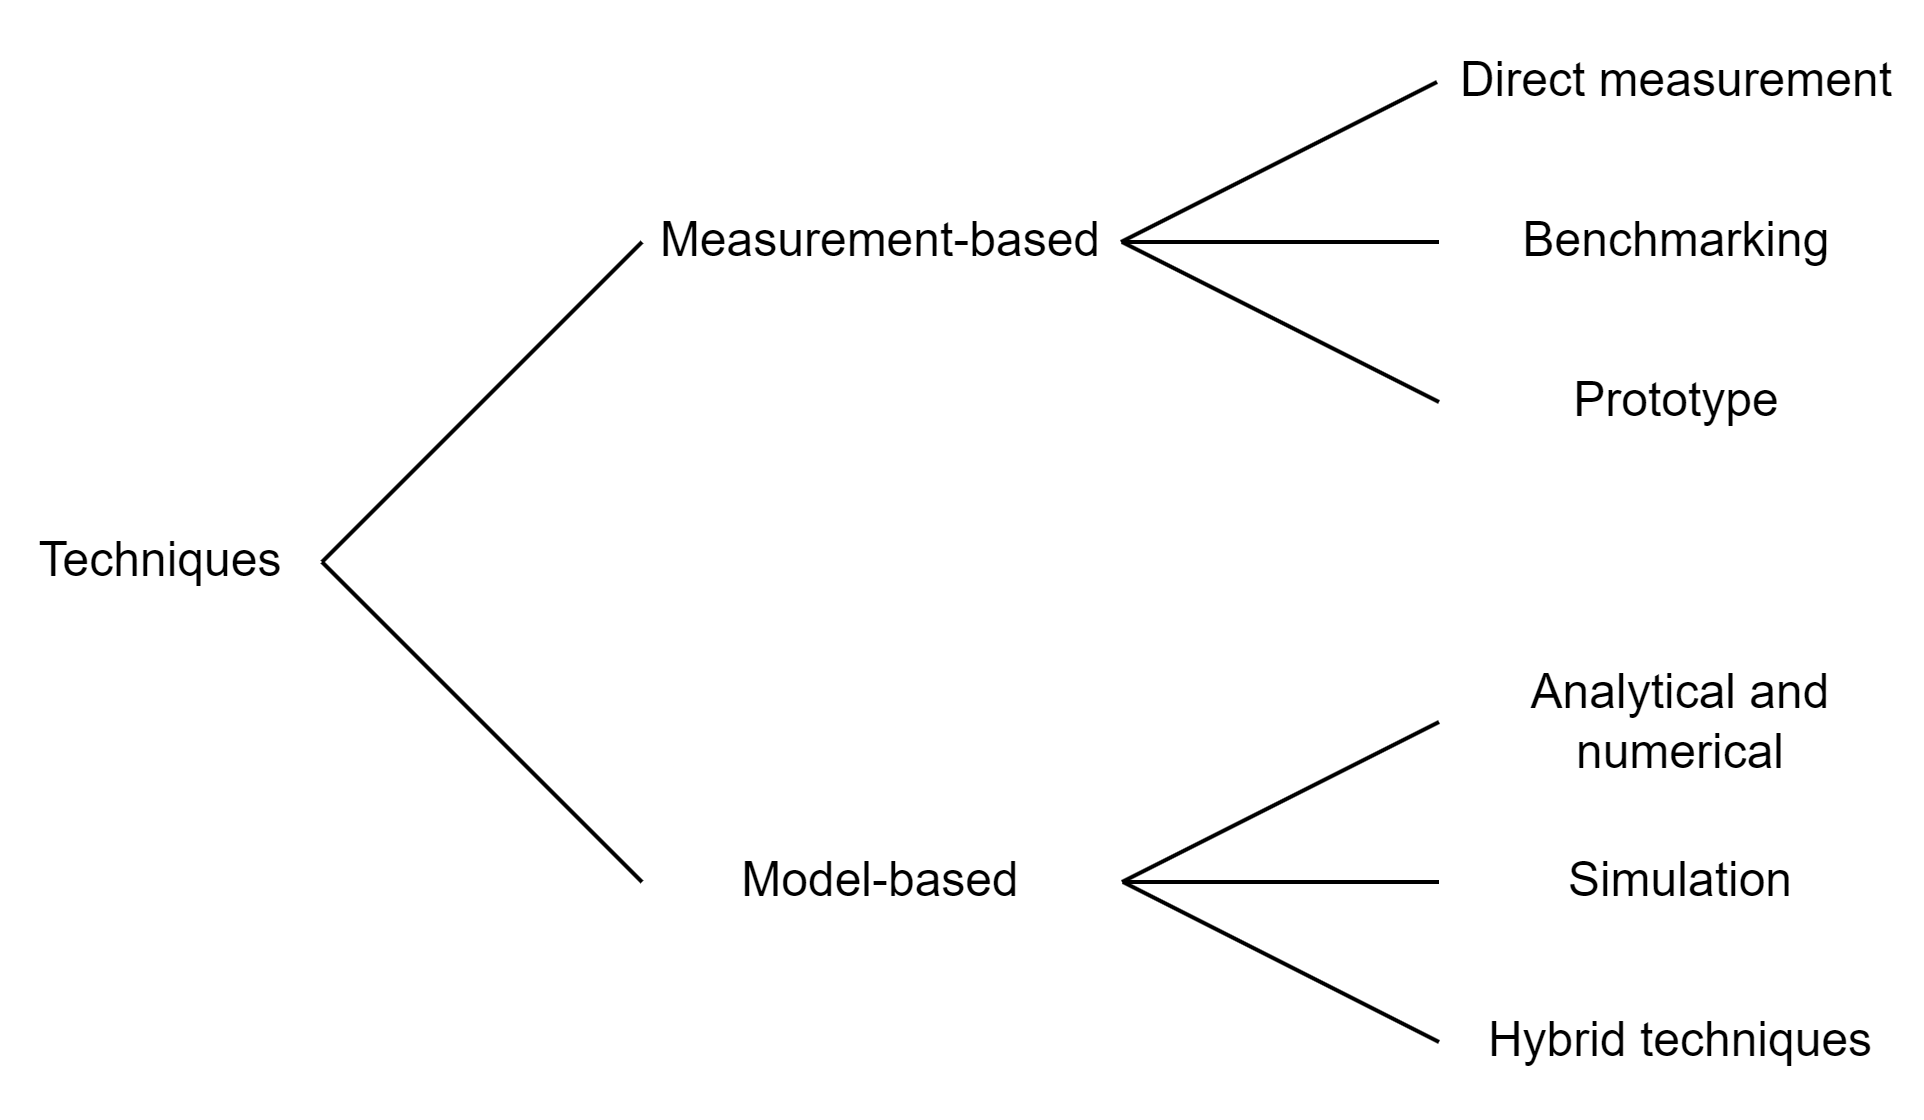
\includegraphics[width=0.5\linewidth]{images/eva.png}
    \caption{Quality evaluation techniques}
\end{figure}

\subsection{Model-based approach}
Due to the complexity of systems, abstraction through modeling is necessary.

\begin{definition}[\textit{Model}]
    A model is a simplified representation of a system that captures its essential features while being less complex than the actual system.
\end{definition}
Models are valuable for predicting and evaluating system behavior.
\begin{figure}[H]
    \centering
    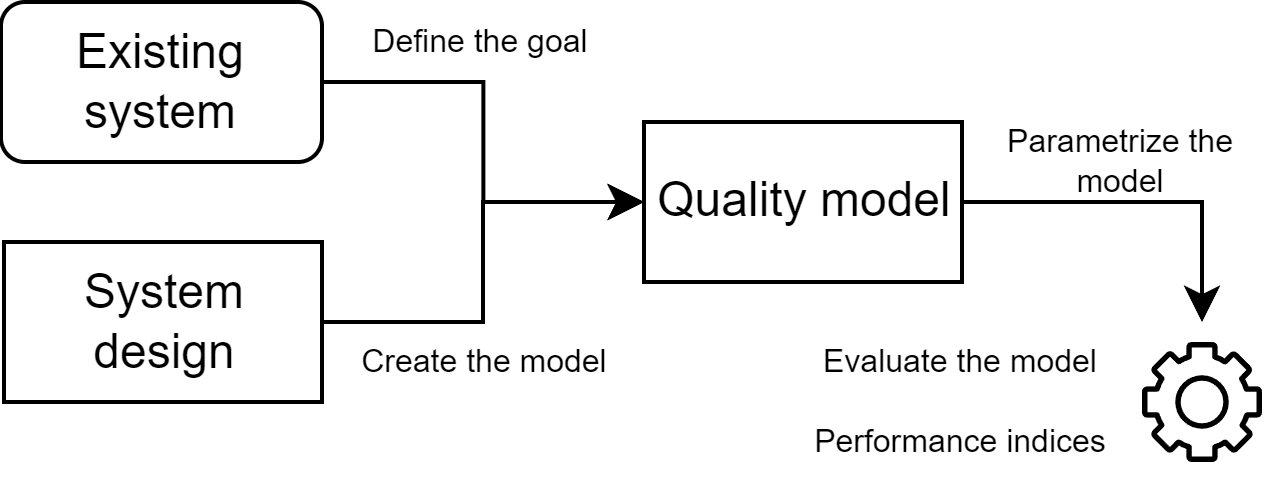
\includegraphics[width=0.5\linewidth]{images/model.png}
    \caption{Model definition}
\end{figure}

The main model-based techniques include:
\begin{itemize}
    \item \textit{Analytical and numerical methods}: these rely on mathematical techniques, often utilizing probability theory and stochastic processes.
        They are highly efficient and precise but tend to be very specific.
    \item \textit{Simulation}: this involves replicating the behavior of the model.
        Simulations are versatile but may lack accuracy in scenarios involving rare events.
        Achieving high accuracy can also result in lengthy solution times.
    \item \textit{Hybrid methods}: these combine analytical or numerical methods with simulation, leveraging the strengths of both to address various aspects of the system.
\end{itemize}